\begin{refsection}

The methodology followed for the development of this project is divided into the experimental and computational methodology. Within the experimental part (Section \ref{sec:exp_methodology}) an explanation on how OS polymer films were done is going to be stated, as well as how performance tests (oxidative TGA and Headspace test) on the oxygen uptake capacity of linseed oil and the oxygen scavenging film were made. Next, the methodology regarding the computational part of the project is described in section \ref{sec:computational methodology}. In this part, an explanation of the mathematical models which describe the physics of the oxygen uptake on the OS film was made. Afterwards, to be able to use the mathematical model obtained to predict the behavior of the OS films, different numerical finite difference methods were studied. Each one of this is going to be disclosed in section \ref{subsec:numerical_methodology.}. Later, a methodology of adjustment following the Gauss-Newton method for the kinetic velocity constants an initial concentrations of linseed oil autoxidation is explained in section \ref{subsec:model_desc.}. Finally, the methodology regarding the design tool interface programming is described in section \ref{sec:metodologia_interfaz}. 
 

\section{Experimental methodology}\label{sec:exp_methodology}
The next section will describe how the PP films with microcapsules containing linseed oil (which is the object of study in this project) are made and how the evolution of oxygen concentration in headspace is going to be measure. Also the methodology regarding the oxidative thermogravimetric analysis made to follow the oxidation kinetics of linseed oil is going to be described. 

\subsection{Silica microcapsules synthesis}\label{sec:capusules}
Regarding the microcapsule synthesis, this has been carried out by the CIPP-CIPEM using the sol-gel emulsion templating methodology. This methodology consists of preparing an emulsion in which the disperse phase is the chemical specie that is desired to be encapsulated. In this case, the surfactant or emulsifier will serve as a template where TEOS precursor undergoes hydrolysis and condensation reactions to form the silica polymeric microcapsule \cites{GonzalezPungo2018EvaluacionActivos, GomezAlfonzo2018AceiteOxigeno} To obtain 2.34g of dry product, initially 85.5 mL of water, 0.48g of cetrimonium bromide (CTAB) and 36mL of ethanol are mixed in a 250mL beaker at a speed of 700rpm during 5 minutes. Afterward, 1.5 mL of double-cooked linseed oil is added drop by drop to the previous mix, and immediately after, 3mL of Tetraethyl orthosilicate (TEOS) is slowly added to the beaker, which is left mixing during 15 minutes more. Finally, 3mL of ammonia is added to the beaker to catalyze the reaction, which is left mixing for 24 hours. The solid obtained is vacuum filtered and dried in a vacuum oven at 50\degree C and a pressure of $-0.06 MPa$ for 4 hours. After that time, the microcapsules are ready to be incorporated into the polymeric film. Next, an image of the product obtained is shown in figure \ref{fig:capsules}. 

\begin{figure}[ht]
    \centering
    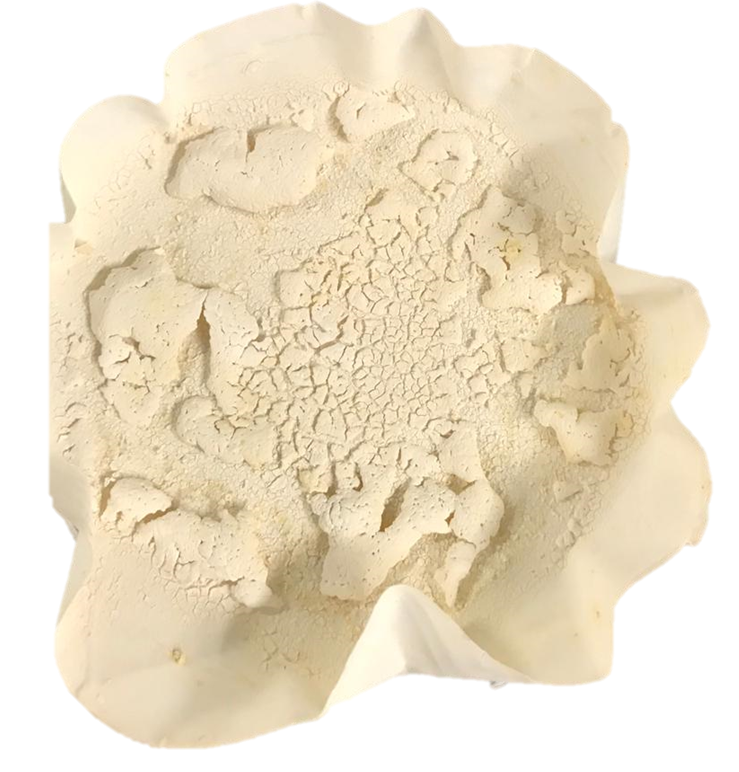
\includegraphics[width=0.3\linewidth]{Documento_Latex/Tesis_1/Imagenes/capsulas.png}
    \caption{Silica microcapsules obtained by the methodology described in section \ref{sec:capusules}}
    \label{fig:capsules}
\end{figure}

\subsection{Film Elaboration} \label{sec:film_elaboration}
Once having 9g of nanocapsules, a masterbatch is prepared by mixing the nanocapsules load and polypropylene-maleic anhydride graft copolymer (PP-g-MAH) in a  20:80 mass proportion respectively. Before entering the sample into the internal mixer, this has to be preheated for 10 minutes so that it reaches a temperature of 190\degree C, after which the mix is poured and stays within 7 minutes at a speed of 60rpm. The material obtained must then be frozen to a temperature of -80\degree C for 3 hours. Afterward, it has to be taken into a blade mill for grinding for 2 minutes and in this way, the masterbatch is ready to be mixed with polypropylene homo-polymer (PP) to form the films. The quantity of masterbatch used is so that the nanocapsule load is 5\% of the total film weight. These two components go again through the same process of mixing as the masterbatch did. Finally, the process of compression molding is done by using a press. To do this, two aluminum foils and two Teflon foils are put over the two sides of the press, and in the inferior part of it, a quantity of 12g of the PP mixture is poured using a 19cm x 19cm x 3cm aluminum frame. The inferior and superior plates are both preheated to a temperature of 190\degree C and the press must be configured so that an initial pressure of 15 bar is applied during 1 minute and then a pressure of 110 bar must be applied during 1.5 minutes after which a 10 minutes cooling time is done. After this, the desired film of 19cm x 19cm with OS load is obtained (Figure \ref{fig:film}).

\begin{figure}[ht]
    \centering
    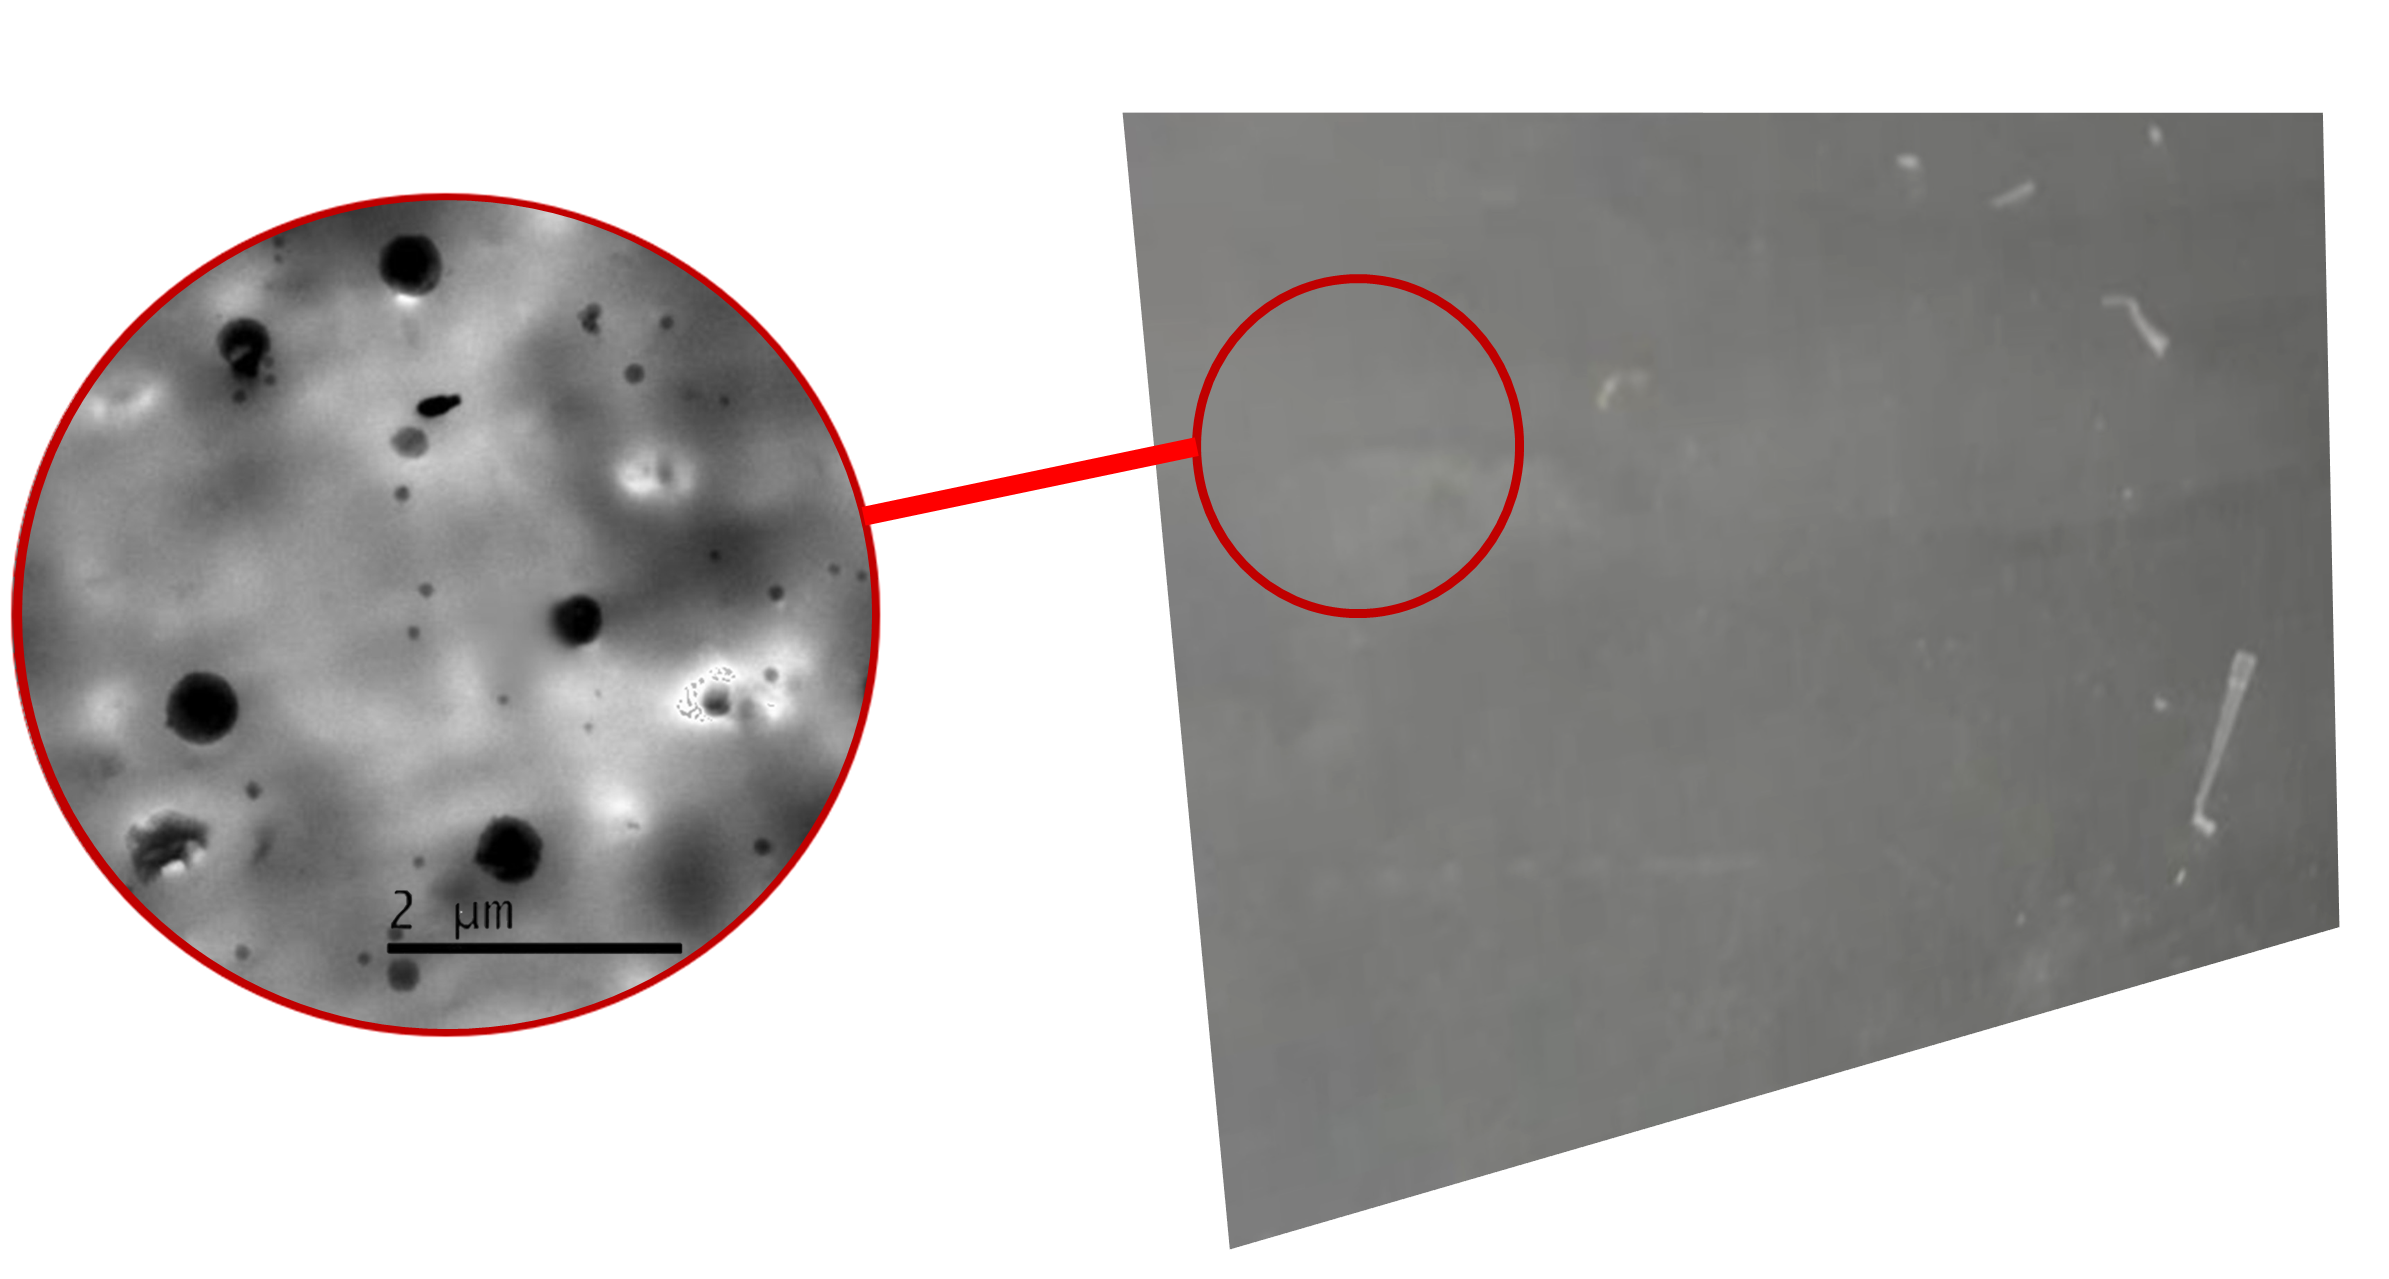
\includegraphics[width=0.6\linewidth]{Documento_Latex/Tesis_1/Imagenes/pelicula.png}
    \caption{PP film containing silica microcapsules which were incorporated by the methodology described in section \ref{sec:film_elaboration} \cite{ArellanoAyala2019EfectosAntioxidantes}}
    \label{fig:film}
\end{figure}

\subsection{Headspace Oxygen Absorption Test}\label{subsec:headspace}
Head-space oxygen absorption is one of the two tests which enables to study the performance of the OS film, and its results together with the oxidative TGA are the ones that are used to verify the prediction capacity of the model proposed. To do this test, a Quantek 901 head-space oxygen analyzer was be used. First, a sample of the film made is placed within a 100mL glass bottle. This bottle is sealed by pressurizing its cap, after which it is ready to test. To perform the test, in the cap of the bottle, a plastic seal will be put and perforation with a needle will be made through it (See Figure \ref{fig:headspace}).

\begin{figure}[ht]
    \centering
    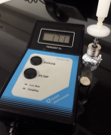
\includegraphics[width=0.25\textwidth]{Imagenes/headspace.png}
    \caption{Headspace oxygen absorption test}
    \label{fig:headspace}
\end{figure}

The gas extracted from the bottle goes by a syringe to a ''fuel cell" type oxygen sensor, which consists of a diffusion barrier, a sensing electrode made of platinum and a working electrode made of zinc, all submerged in a solution of potassium hydroxide which acts as an electrolyte \cite{Boissevain1996CorporateGuide}. The entering oxygen diffuses into the sensor a reduces to hydroxyl ions at the cathode.

 \reaction{O2 +2H2O +4e^- -> 4OH^-}
the hydroxyl ions formed are oxidized at the zinc anode.
 \reaction{2Pb + 4OH^- -> 2PbO +2H2O + 4e^-}
 which yields an overall cell reaction 
 \reaction{2Pb + O2 -> 2PbO}

 
 The current generated during this reaction is proportional to the concentration of oxygen present in the medium. With this in mind,  the sensor measures these currents and calculates the quantity of oxygen within the air \cite{GarciaMora2015KineticScavengers, Boissevain1996CorporateGuide}. This test was carried out every 12 hours until the oxygen concentration becomes constant in time, which indicates that the oxygen absorption on behalf of the film has stopped and so its useful life. It is essential to mention that for avoiding external air for entering the vial, each one of this was punctured once, and then it was discarded. Negative control was carried out for each head-space test done. For every puncture made, a  quantity of 4 ml of air is extracted from the bottle; this was calibrated, taking into account the advice from the manufacturer. The analyzer Quantek model 901 has a resolution of 0.1\% and an accuracy of $\pm$0.1\% in reading \cite{Instruments2019ModelAnalyzer}. 
 
\subsection{Oxidative TGA}
The second oxygen uptake performance test, which was made on OS films and linseed oil individually, is a thermogravimetric analysis (TGA). Given that in the autoxidation process described in Section \ref{subsec:PUFA_os}, there is an increase in the weight of oils due to the absorption of oxygen from the environment. Even though these changes in weight are minimal, they are big enough for being detected in the thermogravimetric analysis. So to determine the performance of the films and the oil, three TGA must be carried out. All tests were made using an SDT Q600 (TA instruments) with isothermal curves at 40\degree C, 60\degree C, 80\degree C, and 110\degree C and a heating rate of 20\degree C/min with a sample mas of 4 mg. The first TGA test carried out was under a nitrogen atmosphere. This is done to observe the sole effect of the flow of air around linseed oil and OS films. In this case, the volatile components within the sample are going to evaporate, generating a reduction in the measured mass. The second TGA test, which has to be carried is in a pure oxygen atmosphere. This is the case in which oxygen is in excess concerning the substrate, so the kinetics of oxidation can be simplified, as explained in section \ref{subsec:PUFA_os}. The results in the change of mass of the sample obtained are normalized for the mass reduction due to the evaporation obtained from the nitrogen atmosphere TGA. In this way, there is a guarantee that the changes observed in the mass on the oxygen TGA are exclusively due to the absorption of oxygen. The third and final TGA made was in air atmosphere, in which oxygen has a concentration of 21 vol\%. Contrary to the case of oxygen atmosphere TGA, in this case, it is not correct to assume that oxygen is in excess to the substrate in the oil, so the results obtained in this test must be compared to the complete autoxidation kinetics of the linseed oil.   

\section{Computational Methodology}\label{sec:computational methodology}
In this section of the document, an explanation of how the development of the computational tool was made is described. The first step taken towards fulfilling this objective was using conservation equations to establish a PDE which describes the dynamics of oxygen within linseed oil and OS polymeric films, this was developed both for monolayer films and for the multilayer films. Therefore, to evaluate the validity of the model developed, a new adjustment of the kinetic constant and initial concentrations was made over linseed oil kinetics. Once having determined the kinetic constants that describe the oxidation of linseed oil, a study of different numerical methods was made to find out which of these enabled a fast and accurate solution of the differential equations established from the mathematical models. Finally, once studied the method by which the model is solved, a graphic interface was developed so that an external user may study the effect of different parameters on the $O_2$ absorption. An explanation of how this interface was made is explained at the end of this section. 

\subsection{Model Description}\label{subsec:model_desc.}

\subsubsection{Mono Layer Film}
The main idea in developing a model that describes the oxygen uptake by an OS film is to replicate the results obtained experimentally by the Headspace oxygen test described in section \ref{subsec:headspace}. To establish this model, a film of Area $A$ and thickness $L$, which is inside a bottle volume $V$ and at constant temperature $T$ is considered. The gas in the bottle considered has an initial oxygen molar concentration $C_{ext_o}$. The situation described is shown in figure \ref{fig:model_diagram}. 

\begin{figure}[ht]
    \centering
    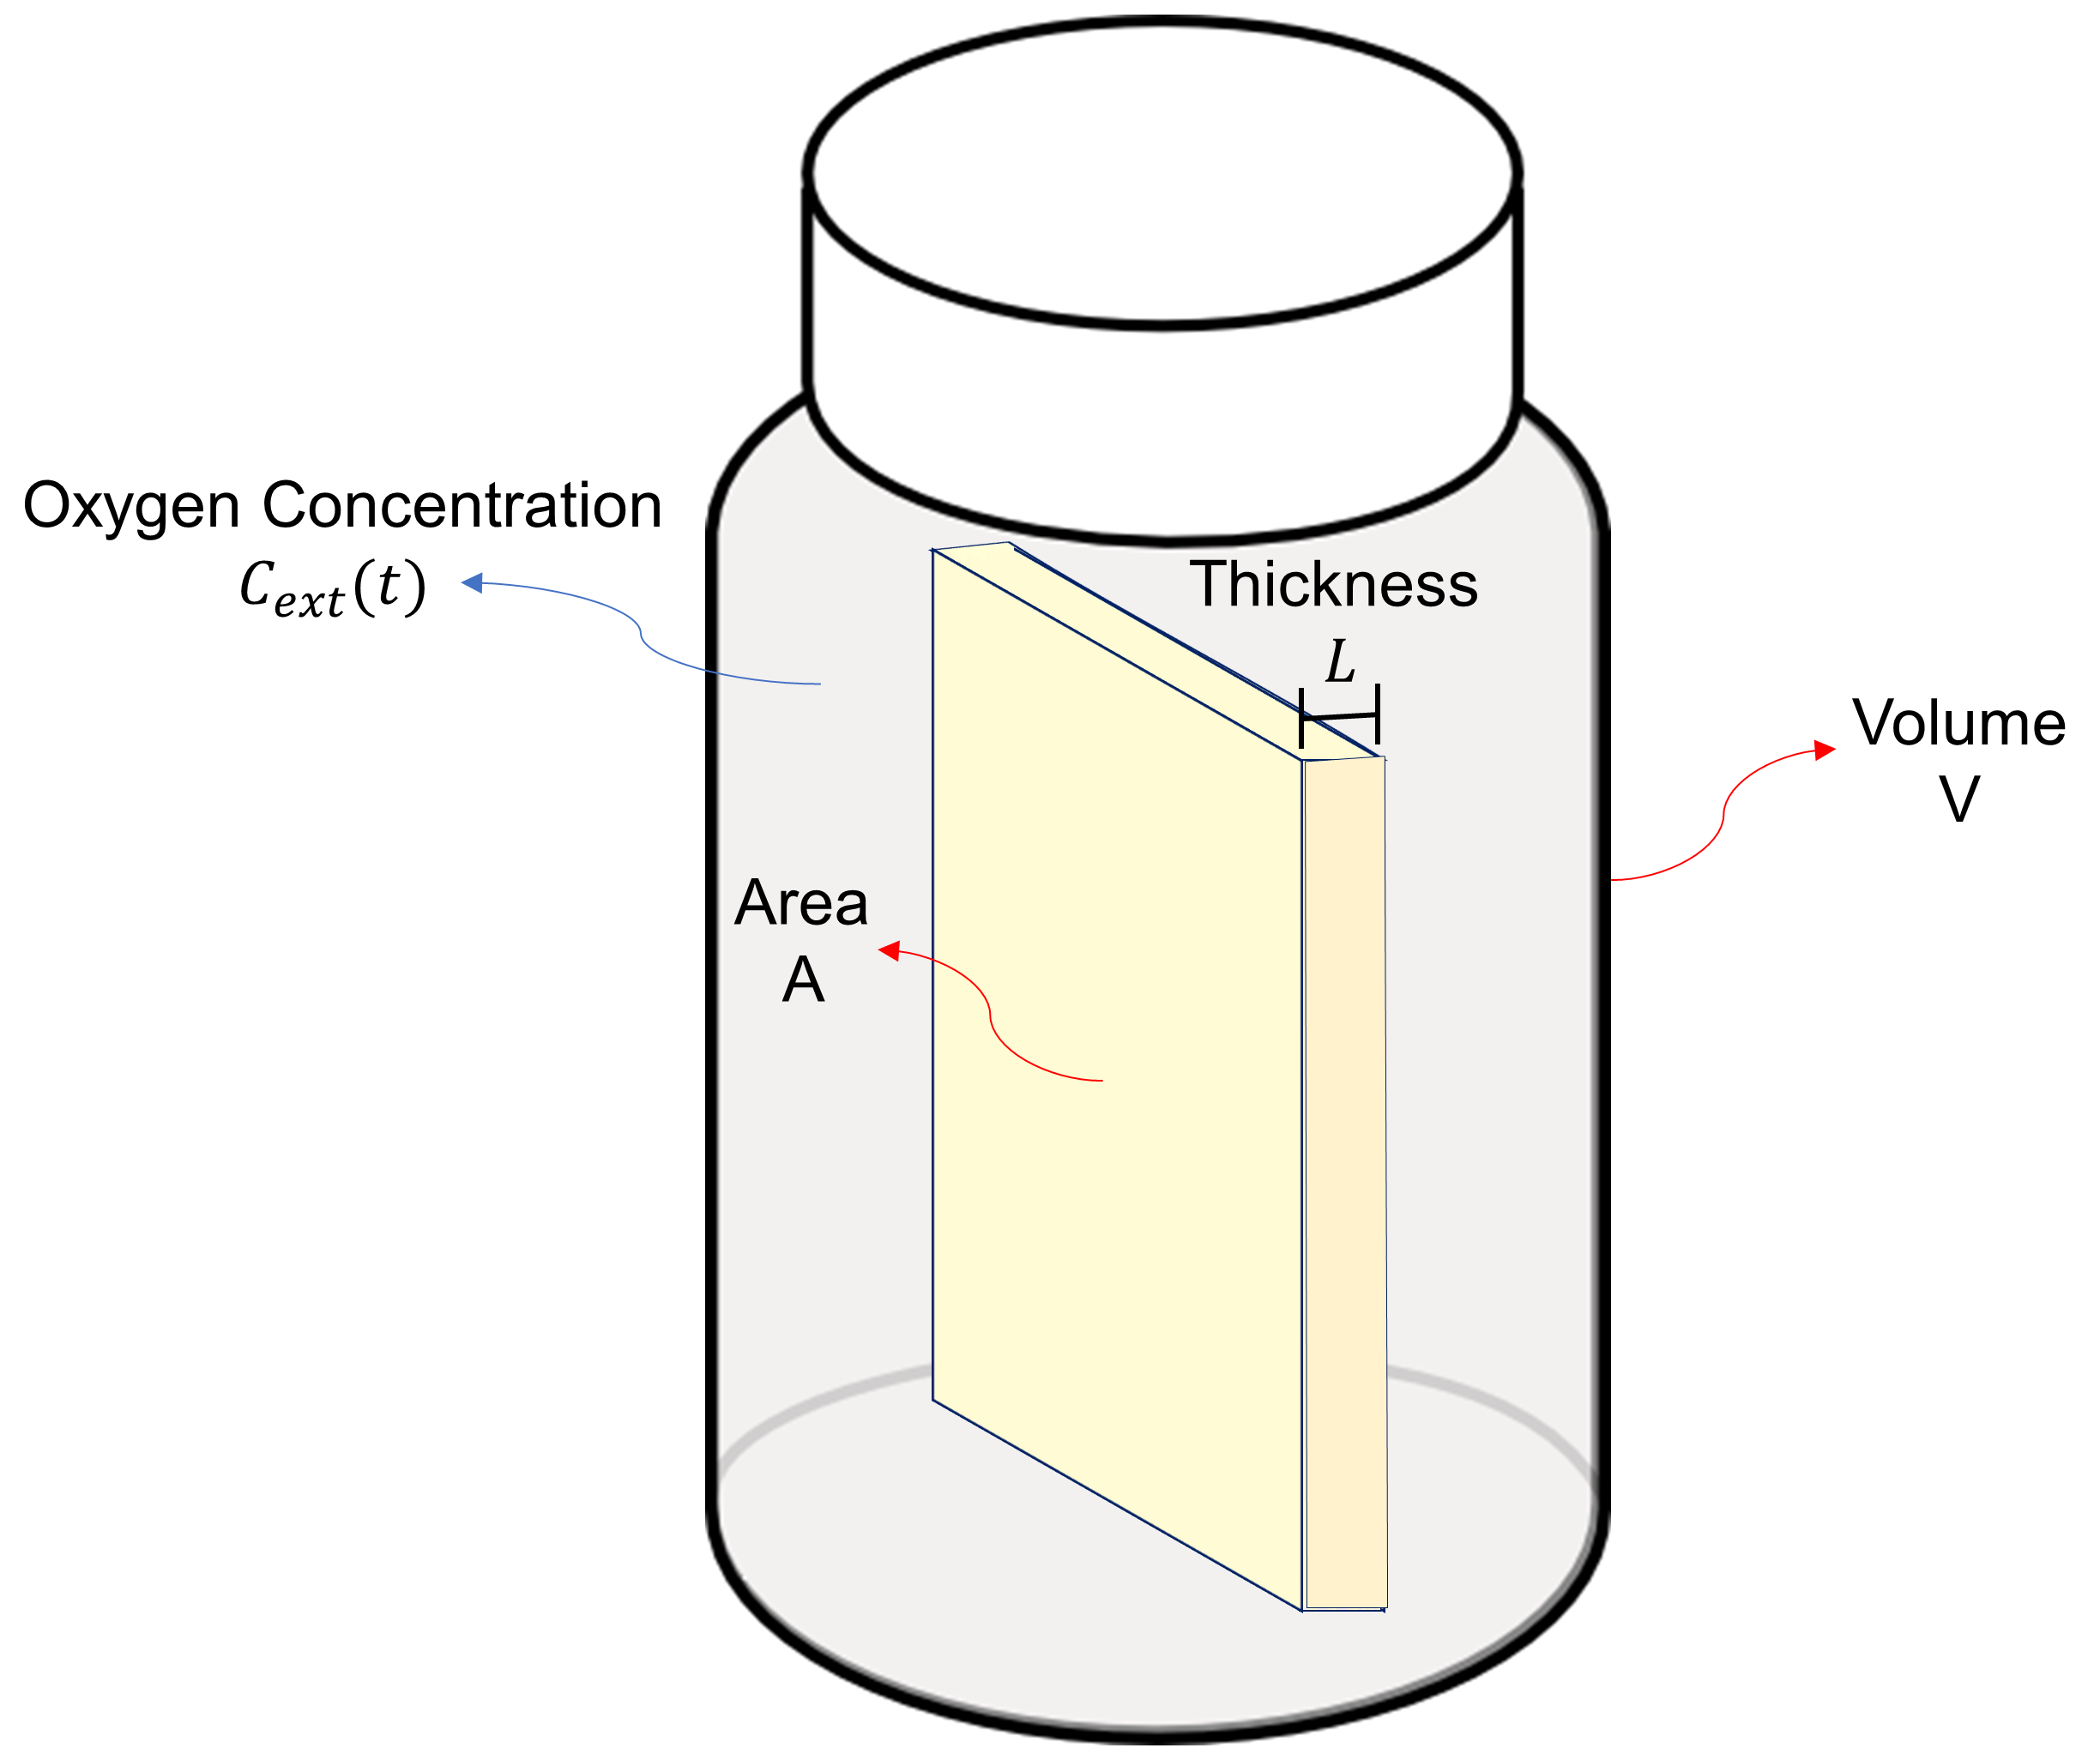
\includegraphics[width=0.5\linewidth]{Documento_Latex/Tesis_1/Imagenes/modelo.png}
    \caption{Schematic diagram of the OS film in a vial with oxygen concentration $C_{ext}$}
    \label{fig:model_diagram}
\end{figure}

In this case, the homogeneous film approach is going to be used. This considers the whole film as reactive with an initial OS volumetric concentration $C_{OS_0}$. For the initial conditions of the model, it was assumed that there is no oxygen consumption or diffusion in the process of compression molding, which is why the initial molar concentration of oxygen in the film is $[O_2]=0 \hspace{5pt} mol/cm^3$.  It is essential to state that in this model, oxygen will be assumed to enter by both faces of Area $A$ and given that this area is much bigger than the thickness $L$ of the film, then the propagation of oxygen into the foil can be assumed to be one dimensional in the direction normal to its faces (Figure \ref{fig:model_diagram}).

Now assuming that the film is isotropic, the diffusion of oxygen through it is going to be given by Fick's first law, which allows calculating the molar diffusive flux as the product of the diffusivity of oxygen in the polymer and the gradient of the $O_2$ concentration within the film (Equation \ref{eq:flux}).

\begin{equation}
    J=-D_{O_2}\nabla [O_2] \xrightarrow{1D}J_x=-D_{O_2}\frac{\partial [O_2]}{\partial x}
    \label{eq:flux}
\end{equation}

In the previous equation, $J$ represents the molar flux of oxygen and $D$ is the diffusivity of oxygen in the polymer material which the film is made of. The equation stated before indicates that the flux will go in the direction in which the concentration of $O_2$ decreases; this suggests that the mass will move towards reducing the concentration gradient in the system. Now, applying this to the oxygen molar balance, the equation \ref{eq:mass_bal_dif} is obtained. 

\begin{equation}
    \frac{\partial [O_2]}{\partial t}= -\nabla \cdot J= \frac{\partial}{\partial x} \left(D_{O_2}\frac{\partial [O_2] }{\partial x}\right)
    \label{eq:mass_bal_dif}
\end{equation}

This last equation is the transient diffusion equation and describes how any species propagates in a medium given a gradient in its concentration. In this case, given that the film is assumed to be reactive, a source/sink term must be taken into account in the prior equation due to the consumption of oxygen by the OS.

\begin{equation}
    \frac{\partial [O_2]}{\partial t}= \frac{\partial}{\partial x} \left(D_{O_2}\frac{\partial [O_2] }{\partial x}\right)+ R
    \label{eq:mass_bal_dif_reacc}
\end{equation}

The equation \ref{eq:mass_bal_dif_reacc}, corresponds to the one dimensional transient diffusion-reaction equation, in which $R$ represents the reactive term. By describing mass conservation in the system with equation \ref{eq:mass_bal_dif_reacc}, there is an assumption that no convection occurs within the vial so there is no net flow of the oxygen in the polymeric film and the only movement of this specie is given by concentration gradients. Now to describe the reactive term shown in the last equation, the kinetic model presented by Garcia \cite{GarciaMora2015KineticScavengers} for describing linseed oil autoxidation is going to be used with a modification on the termination equation of peroxyl radicals (this modification is explained in section). This model assumes that the reactions which occurs during oxidation are:

\reaction[reacc:initiation]{2ROOH ->[k_1] ROO^. +R^. + carbonyl + Scission}
\reaction[reacc:O_2 consumption]{R^. + O2 ->[k_2] ROO^.}
\reaction[reacc: propagation]{ROO^. + RH ->[k_3] ROOH + R^.}
\reaction[reacc:termination_2alkyrad]{R^. +R^. ->[k_4] $\text{Inactive Products}$}
\reaction[reacc:termination_alky_peroxide_rad]{R^. +ROO^. ->[k_5] $\text{Inactive Products}$}
\reaction[reacc:termination_2peroxide_rad]{ROO^. +ROO^. ->[k_6] $\text{Inactive Products}$}

Where $ROOH$ is hydroperoxide, $RH$ is the substrate and \ce{R^.}, \ce{ROO^.} are the alkyl and peroxyl radicals respectively. By assigning a simple kinetics using the rate law expression the following system of ordinary differential equations (ODE) is obtained:

\begin{gather}
    \frac{d[\ce{R^.}]}{dt}= k_1[ROOH]^2 - k_2 [\ce{R^.}][O_2]+ k_3[\ce{ROO^.}][RH]-2k_4[\ce{R^.}]^2 -k_5[\ce{R^.}][\ce{ROO^.}]\label{eq:consum_R.}\\
    \frac{d[\ce{ROO^.}]}{dt}= k_1[ROOH]^2 + k_2 [\ce{R^.}][O_2]- k_3[\ce{ROO^.}][RH]-k_5[\ce{R^.}][\ce{ROO^.}]-2k_6 [ROO^.]^2\\
   \frac{d[ROOH]}{dt}= -2k_1[ROOH]^2 + k_3[\ce{ROO^.}][RH]\\
   \frac{d[RH]}{dt}=-k_3[\ce{ROO^.}][RH]\label{eq:consum_RH}\\
   \frac{d[O_2]}{dt}= -k_2[\ce{R^.}][O_2]\label{eq:consum_O2}
\end{gather}

Combining the equations \ref{eq:mass_bal_dif_reacc} and \ref{eq:consum_O2}, the oxygen mass balance can be expressed as:

\begin{equation}
     \frac{\partial [O_2]}{\partial t}= \frac{\partial}{\partial x} \left(D_{O_2}\frac{\partial [O_2] }{\partial x}\right) -k_2[\ce{R^.}][O_2].
    \label{eq:mass_bal_def}
\end{equation}

This last equation together with equations \ref{eq:consum_R.} to \ref{eq:consum_RH} are going to describe the dynamics of oxygen concentration within the film. Also, this are the ones that are going to be numerically solved (this is going to be explained in section \ref{subsec:numerical_methodology.}). On the other hand, the total quantity of oxygen absorbed by the film is calculated by integrating the mass flow of oxygen into it. 

\begin{equation}
    m_{O_2}(t)= \int_0^t \dot{m}dt =M_{O_2}A\int_0^t Jdt 
\end{equation}

To arrive at the right-hand side of the equation, mass flux was calculated by multiplying the molar flux $J$ by the molecular weight of oxygen $M_{O_2}$, while the mass flow was calculated by multiplying the mass flux by the film area $A$. It is essential to state that the flux $J$ used to calculate the total mass of oxygen in the film is the sum of the flux at both faces of the film, $J= J_x\rvert_{x = 0} - J_x\rvert_{x = L}$. But given that the concentration $[O_2]$ is symmetrical concerning the film, the flux at both faces will be equal in magnitude, so $J=2J_x\rvert_{x = 0}$.  Now replacing the definition of molar flux (Equation \ref{eq:flux}) into the previous expression

\begin{equation}
    m_{O_2}(t) =-2D_{O_2}AM_{O_2}\int_0^t \frac{\partial [O_2]}{\partial x}\biggr\rvert_{x = 0}dt
    \label{eq:total_mass_O2}
\end{equation}

This last expression will enable to calculate the oxygen uptake profile through time as well as the head space oxygen concentration profile (Equation \ref{eq:headspace}). 

\begin{equation}
    C_{ext}(t)= C_{ext_o} - \frac{1}{M_{O_2}V} m_{O_2}(t)= C_{ext_o} + \frac{2AD_{O_2}}{V} \int_0^t \frac{\partial [O_2]}{\partial x}\biggr\rvert_{x = 0}dt
    \label{eq:headspace}
\end{equation}

This last quantity, $C_{ext}(t)$, is of great interest,
because it is the one that the headspace test
allows to obtain experimentally, so the model
will seek to predict the behavior of this quantity
overtime. Concerning the initial and boundary conditions in this problem, as stated at the beginning of this section the film is going to be considered to be devoid of $O_2$ and the external headspace oxygen concentration is going to be $C_{ext_o}$. Also concerning the initial concentration of the reacting species in the linseed oil (i.e. hydroperoxide,substrate, alkyl, and hydroxyl radicals) is it assumed that they are going to be uniform through the whole film (Equation \ref{eq:ic_mono_film}). 

\begin{align}
    &\text{IC: } & &[O_2](x,t=0)=0, & &C_{ext}(t=0)= C_{ext_o},\nonumber\\
    && &[\ce{RH}](x,t=0)=C_{OS}[\ce{RH}]_o,   & &[\ce{ROOH}](x,t=0)=C_{OS}[\ce{ROOH}]_o, \nonumber\\
    && &[\ce{R^.}](x,t=0)=C_{OS}[\ce{R^.}]_o,   & &[\ce{ROO^.}](x,t=0)=C_{OS}[\ce{ROO^.}]_o. 
    \label{eq:ic_mono_film}
\end{align}
    
The quantities $[\ce{RH}]_o$, $[\ce{ROOH}]_o$,  $[\ce{R^.}]_o$, and $[\ce{ROO^.}]_o$ are the respective molar concentrations of chemical species in Linseed oil and $C_{os}$ is the charge of OS scavenger in the film. This latter quantity is calculated by multiplying the mass charge of OS in the film (wt\%) by the reason between the oil and the film density (Equation \ref{eq:load_concentration}).

\begin{equation}
    C_{OS}= \text{Oil wt}\% \frac{\rho_{polymer}}{\rho_{oil}}
    \label{eq:load_concentration}
\end{equation}

On the other hand, given that the molar balance of oxygen in the film has second-order derivative respect to the spatial component, it is necessary to establish two boundary conditions over the film so that the problem stated has a solution. These conditions are given in the outer face of the film, which is in contact with the head-space gas. In this case, oxygen dissolved in the boundary face of the film must be in equilibrium with the external oxygen. This equilibrium is described by Henry's law which states that the partial concentration of the oxygen dissolved in the polymer is proportional to the partial pressure of oxygen in the head-space gas (i.e. $[O_2](x=0, L)=s\hspace{2pt}p_{O_2}$ ). The relation between the partial pressure of oxygen and its'external concentration is obtained assuming that the gas in the vial behaves as an ideal gas.  In that case $p_{O_2}=RTC_{ext}(t)$, and so the boundary conditions for oxygen concentration in the film are:

\begin{align}
    &\text{BC:} & &[O_2](x=0, t)= \left(sRT\right) C_{ext}(t) & & [O_2](x=L, t)= \left(sRT\right) C_{ext}(t)
    \label{eq:bc_mono_film}
\end{align}

With these set of initial and boundary conditions, the complete set of conditions necessary to solve the problem is established.

\subsubsection{Multi-layer Film}
Continuing with the presentation of the mathematical models developed for the creation of an OS film modeling tool, the case of a multilayer system was considered. The situation studied was a multilayer OS film with total thickness $L$,  composed of  $n$ layers, each one of thickness $L_i, 0<i<n$ where  $L_i\neq L_j, \forall  i\neq j$ and made of a different material. The film has a face of area $A$ and is inside a vial of volume $V$ with an initial headspace oxygen concentration $C_{ext_o}$. The situation described is shown in figure \ref{fig:model_multilayer_diagram}.

\begin{figure}[ht]
    \centering
    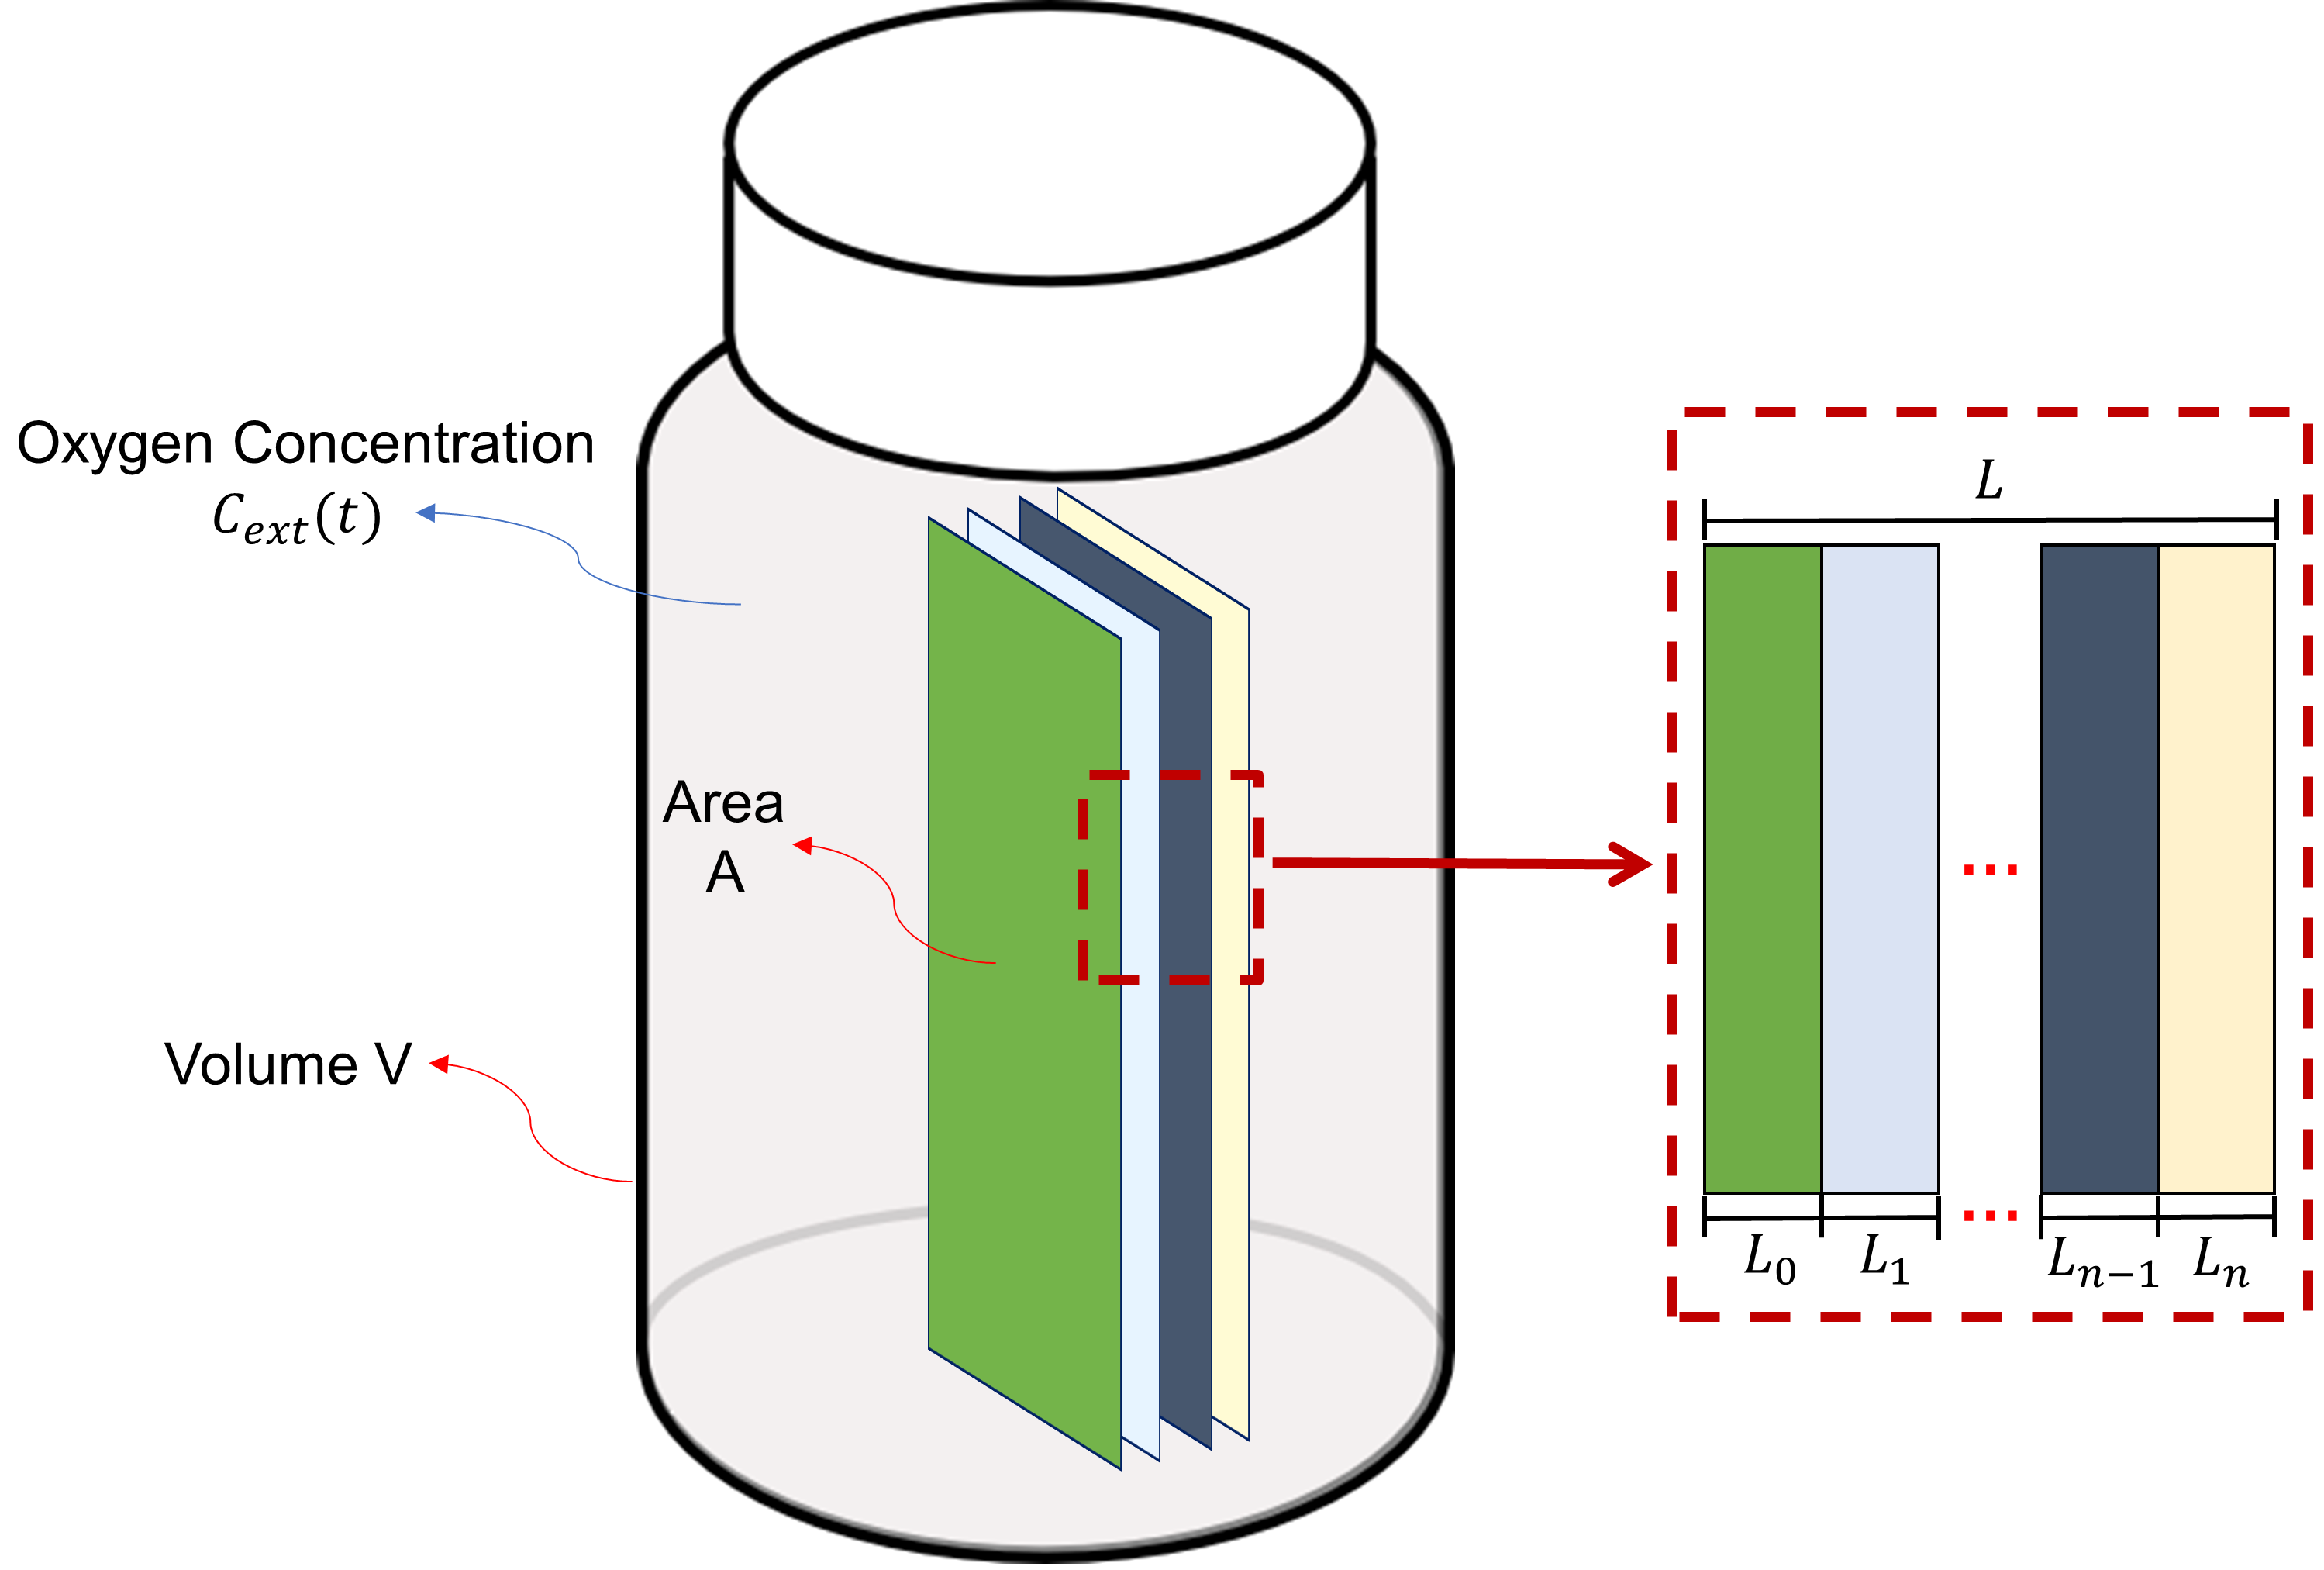
\includegraphics[width=0.62\linewidth]{Documento_Latex/Tesis_1/Imagenes/modelo_multicapa.png}
    \caption{Schematic diagram of a OS film composed of $n$ different layers in a vial with oxygen concentration $C_{ext}$}
    \label{fig:model_multilayer_diagram}
\end{figure}

The equation describing the dynamics of the reaction in the film are the same as equations \ref{eq:consum_R.} to \ref{eq:consum_RH}, while the expression regarding oxygen concentration dynamics in the film is going to be

\begin{equation}
    \frac{\partial [O_2]}{\partial t}= \frac{\partial}{\partial x} \left(D_{O_2}(x) \frac{\partial [O_2] }{\partial x}\right) -k_2[\ce{R^.}][O_2]
    \label{eq:mass_bal_def_multi}
\end{equation}

The main difference between the last equation and equation \ref{eq:mass_bal_def} is that the diffusivity of oxygen depends on the position $x$ in the film. The function that describes this dependence is :

\begin{align}
    D_{O_2}&=  D_i,  & L_{i-1}&< x< L_i,
\end{align}

where $D_i$ is the diffusivity of oxygen in the material of the $i$th-layer of the film. Now, given that the model assumes that all layers are of  different materials, then the flux of oxygen in both faces of the film is not going to be equal, i.e. $J_x\rvert_{x = 0}\neq-J_x\rvert_{x = L} $. This is why in this case the total oxygen mass absorbed by the film has to be calculated as:
\begin{equation}
    m_{O_2}(t) =-AM_{O_2}\int_0^t \left(D_{O_2}(x)\frac{\partial [O_2]}{\partial x}\biggr\rvert_{x = 0} -D_{O_2}(x)\frac{\partial [O_2]}{\partial x}\biggr\rvert_{x = L}\right )dt.
    \label{eq:total_mass_O2_multi}
\end{equation}

And so the headspace oxygen concentration profile is going to be given by:
\begin{equation}
    C_{ext}(t)=C_{ext_o} + \frac{A}{V} \int_0^t \left(D_{O_2}(x)\frac{\partial [O_2]}{\partial x}\biggr\rvert_{x = 0} -D_{O_2}(x)\frac{\partial [O_2]}{\partial x}\biggr\rvert_{x = L}\right) dt.
    \label{eq:headspace_multi}
\end{equation}

Besides the previous equations, there exists an internal boundary condition at the interface between any two collateral layers. This states that the flux of oxygen as well as it's partial pressure are continuous due to mass conservation. The partial pressure of a gas dissolved in a certain media is given by Henry's law, $p=sC$, where $s$ is the solubility of the gas in the media. Given that at the interface of the layer the partial pressure must be continuous:
 \begin{equation}
   p_{i}(x=L_i) =p_{i+1}(x=L_i)  \xrightarrow{}\frac{[O_2]_{i}(x=L_i)}{S_{i}} =\frac{[O_2]_{i+1}(x=L_i)}{S_{i+1}},
 \end{equation} where $p_{i}(x=L_i)$, $[O_2]_{i}(x=L_i)$ and $S_{i}$ is the partial pressure, concentration and solubility of oxygen in $ith$ layer of the film at position $x=L_i$ (which is the interface) and  $p_{i+1}(x=L_i)$, $[O_2]_{i+1}(x=L_i)$ and $S_{i+1}$ are the partial pressure, concentration and solubility of oxygen in the $i+1th$ film of the layer at the interface $x=L_i$. 

Lastly, to establish this model, boundary and initial conditions are necessary. For the latter conditions, this are the same ones established for the monolayer film (Equation  \ref{eq:ic_mono_film}) with the difference that $C_{OS}=f(x)$ (see equation \ref{eq:ic_multi_film}).

\begin{align}
    &\text{IC: } & &[O_2](x,t=0)=0, & &C_{ext}(t=0)= C_{ext_o},\nonumber\\
    && &[\ce{RH}](x,t=0)=C_{OS}(x)[\ce{RH}]_o,   & &[\ce{ROOH}](x,t=0)=C_{OS}(x)[\ce{ROOH}]_o, \nonumber\\
    && &[\ce{R^.}](x,t=0)=C_{OS}(x)[\ce{R^.}]_o,   & &[\ce{ROO^.}](x,t=0)=C_{OS}(x)[\ce{ROO^.}]_o. 
    \label{eq:ic_multi_film}
\end{align}

The reason why in this case $C_{OS}$ depends on the position of film is that not all the layers of the film are reactive. The layers which are inert, have no load of Linseed oil, while reactive layers are. This do not necessarily mean that  all have the same load of Linseed oil (i.e. $C_{OS_i}\neq C_{OS_{j}}, \forall i\neq j$). With this in mind, $C_{OS}(x)$  is given by the following expression:
\begin{equation}
    C_{OS}(x)= 
    \begin{cases}
    0  &\quad\text{if film }i \text{ is inert and } L_{i-1} \le x \ge L_i\\
    C_{OS_i}  &\quad\text{if film }i \text{ is reactive and }  L_{i-1} \le x \ge L_i,\\
    \end{cases}
\end{equation}
where $C_{OS_i}$ (the load of OS per layer) is calculated as:
\begin{equation}
    C_{OS_i}= \text{Oil wt}\%_i \left( \frac{\rho_{polymer_i}}{\rho_{oil}}\right).
    \label{eq:load_multi_concentration}
\end{equation}

On the other hand, the boundary conditions established for the monolayer film (Equation \ref{eq:bc_mono_film}) are valid for the multilayer case, with the difference that the solubility term on each boundary depends on the material of the exterior faces. Having said this, the boundary condition are going to be:
\begin{align}
    &\text{BC:} & &[O_2](x=0, t)= \left(s_0RT\right) C_{ext}(t) & & [O_2](x=L, t)= \left(s_nRT\right) C_{ext}(t),
    \label{eq:bc_multi_film}
\end{align}
where $s_o$ and $s_n$ are the oxygen solubility in the material of the first and last layer of the film. With the boundary and initial conditions established, the model for the multilayer film case is finished. 

\subsection{Numerical Resolution Methodology}\label{subsec:numerical_methodology.}
To obtain a solution to the models presented in section \ref{sec:modeling}, given the complexity of the system of differential equations to be solved, there exists the necessity of using numerical methods. Even though these methods do not enable us to find the exact solution of the problem, it does enables us to obtain an approximation of the analytical solution within an error interval, which depends on the implementation of the solution algorithm. In this case, given that the system of partial differential equations (PDE) which is needed to be solved is one dimensional, this system is going to be solved using finite differences techniques. These methods are based on the approximation of the definition of derivative to a finite difference, which can be solved algebraically (Equation \ref{eq:fin_dif}).

\begin{equation}
    \frac{df}{dx}\approx \frac{f(x_{i+1})-f(x_{i}) }{\Delta x}
    \label{eq:fin_dif}
\end{equation}

To use this technique, the domains in which the equations are going to be solved must be discretized. With this in mind, the spacial domain $x$ in which the diffusion and reaction of oxygen take place becomes $x_i$, which are $n$ discrete points that represent the whole domain. In the same way, time $t$ becomes $t_j$ where $0<j<m$, being $m$ the total number of steps taken in the time interval which is going to be solved. For solving the  system of equations \ref{eq:consum_RH} to  \ref{eq:mass_bal_def}
different finite-difference algorithms were evaluated to find which of these methods was able to solve the diffusion-reaction equation in a fast and stable way. In the next subsections, the methods which were taken into account for this are going to be described, as well as how these were applied to the PDE system of the OS film. 

\subsubsection{Methods of lines}
One of the most straightforward techniques used for numerically solving PDEs is the method of lines (MOL). This method enables to transform a system of PDEs to a system of ODEs, which in turn can be solved using ODE methods such as Runge-Kutta or backward difference formula (BDF), among others. To do this all the dimensions within the PDE equation must be discretized except one. In this case, the equation which is going to be solved is

\begin{equation*}
     \frac{\partial [O_2]}{\partial t}= \frac{\partial}{\partial x} \left(D_{O_2}\frac{\partial [O_2] }{\partial x}\right) -k_2[\ce{R^.}][O_2]
\end{equation*}

The variable which is going to be discretized is $x$ or the spacial dimension. This was chosen given that the only specie which has a spacial component in its mass balance is oxygen, the rest only varies along time. This implies that the reactive sites are fixed within the film. The discretization scheme chosen for the second derivative is a second-order central difference  (Equation \ref{eq:disc_diff}). 

\begin{equation}
    D_{O_2}\frac{\partial^2 [O_2]}{\partial x^2}= D_{O_2} \frac{[O_2]_{i-1}-2[O_2]_{i}+[O_2]_{i+1}}{(\Delta x)^2}
    \label{eq:disc_diff}
\end{equation}

Applying the previous equation into molar balance equation of oxygen the next expression is obtained:
\begin{equation}
     \frac{\partial [O_2]_i}{\partial t}=  D_{O_2} \frac{[O_2]_{i-1}-2[O_2]_{i}+[O_2]_{i+1}}{(\Delta x)^2} -k_2[\ce{R^.}]_i[O_2]_i.
     \label{eq:LOD_oxygen}
\end{equation}
This equation now represents an ordinary differential equation for $[O_2]_i$, which is a vector of variables of concentration of oxygen through the spacial domain which only depends on time (see Figure \ref{fig:LOD_diagram}).

\begin{figure}[ht]
    \centering
    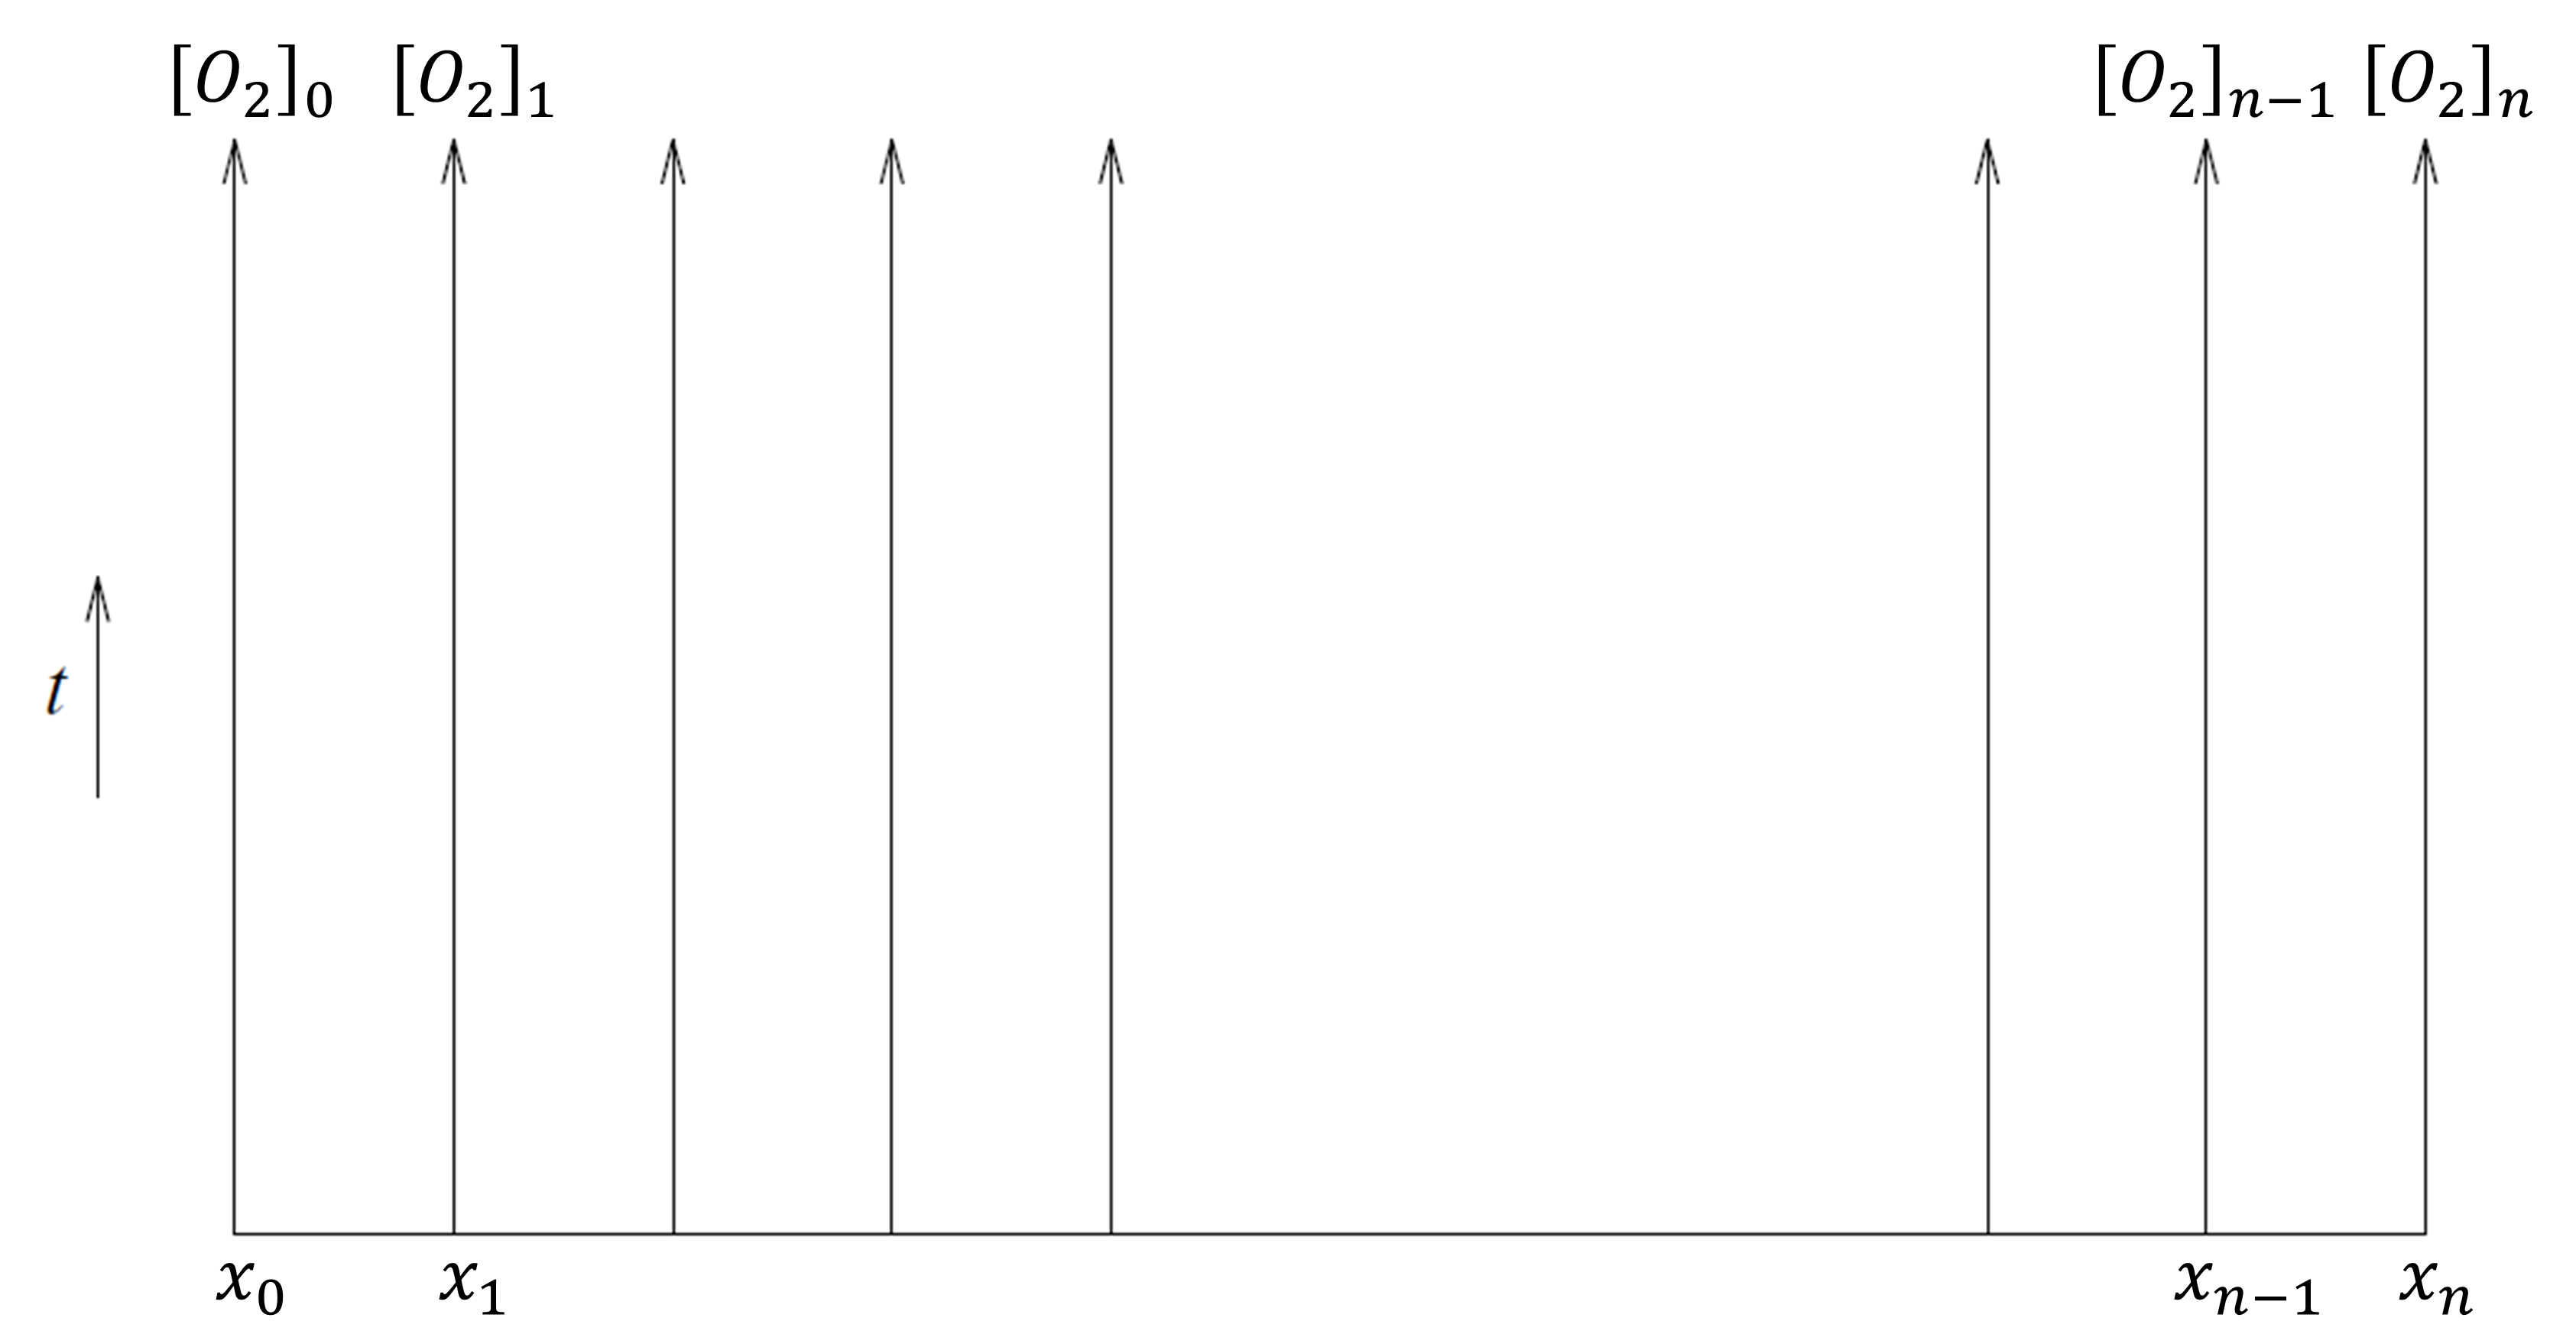
\includegraphics[width=0.7 \linewidth]{Documento_Latex/Tesis_1/Imagenes/LOD.png}
    \caption{Method of lines interpretation. $[O_2]_i$ is the solution along the line forward in time at the grid point $x_i$. Adapted from \cite{LeVeque2007FiniteProblems}.}
    \label{fig:LOD_diagram}
\end{figure}

To solve the system of ODEs, a trapezoidal method will be used. These methods consist of calculating the time derivative at a point $t_i$ as the average of the derivative in that time step and the derivative in the next time step $t_{i+1}$. With this in mind, if the derivative of the oxygen concentration in the film with respect to time is given by equation \ref{eq:LOD_oxygen}, then in the approximation finite difference approximation this derivative is going to be given by:

\begin{align}
    \frac{[O_2]^{j+1}_i-[O_2]^j_i}{\Delta t}=&\frac{1}{2}\Biggr(\left[ D_{O_2} \frac{[O_2]_{i-1}^{j+1}-2[O_2]_{i}^{j+1}+[O_2]_{i+1}^{j+1}}{(\Delta x)^2}-k_2[\ce{R^.}]_i^{j+1}[O_2]_i^{j+1}\right] \nonumber\\
    &-\left[D_{O_2}\frac{[O_2]_{i-1}^{j}-2[O_2]_{i}^{j}+[O_2]_{i+1}^{j}}{(\Delta x)^2}-k_2[\ce{R^.}]_i^{j}[O_2]_i^{j}\right]\Biggr).
\end{align}
This last equation is implicit with respect to time, given that the next time step can not be solve directly from the last step without solving a system of equations. The method implemented was implicit given that it is unconditionally stable and given the presence of the diffusive term which is stiff, an implicit method is required so that the method can be solve using greater time step.  The method of trapezoid when applied to LOD with a second derivative, coincides with the numerical method of Crank-Nicholson. To solve the previous system of equations in order to calculate a new time step, the previous function is rewritten as:

\begin{align}
    0=&\frac{[O_2]^{j+1}_i-[O_2]^j_i}{\Delta t}-\frac{1}{2}\Biggr(\left[ D_{O_2} \frac{[O_2]_{i-1}^{j+1}-2[O_2]_{i}^{j+1}+[O_2]_{i+1}^{j+1}}{(\Delta x)^2}-k_2[\ce{R^.}]_i^{j+1}[O_2]_i^{j+1}\right] \nonumber\\
    &-\left[D_{O_2}\frac{[O_2]_{i-1}^{j}-2[O_2]_{i}^{j}+[O_2]_{i+1}^{j}}{(\Delta x)^2}-k_2[\ce{R^.}]_i^{j}[O_2]_i^{j}\right]\Biggr),
\end{align}
which is equivalent to 
\begin{equation}
    0=F([O_2]^{i+1}). 
\end{equation}
So to find the root for the last equation will mean to calculate the next time step. This was done using the function \textit{fsolve} of the \textit{scipy} library and using as initialization the vector of concentration of the previous time step $[O_2]^{i}$. The initialization was chosen so that the solver converges quickly into a solution given that the profile will not change drastically in one time step. This was done for each time step until the final time $t_m$ was reached. It is important to highlight that both time and space have a uniform discretization. 

\subsubsection{Implicit-Explicit Method}
The implicit-explicit method (IMEX) is a method that has been long used for solving reaction-diffusion problems. This is because generally, the reaction part of the PDE tends to be non-stiff, which is why it can be solved individually by an explicit method, which is simpler to implement and does less work per time step than an implicit scheme. Given that the diffusion part of the equation is stiff, the use of an explicit method to solve the whole PDE is not viable, because it would require excessively small time steps for the method to be stable. In that sense, it is possible to think that an explicit treatment can be given to the reaction part of the PDE, while providing an implicit treatment to the diffusive component of it. In this way, less computational time and effort will be needed to solve the whole PDE given. This is the principle under which IMEX schemes are created. There exist several methods that apply the IMEX schemes; this depends on the treatment given to the implicit and explicit part. In this project, 4 IMEX schemes were evaluated.

The first and most simple IMEX method evaluated was the first order semi-implicit backward differentiation formula (1-SBDF). This scheme is based on the application of the BDF method to solve the diffusive part of the reaction implicitly while using a simple forward Euler method for the reactive part. Applying this algorithm to the oxygen molar balance equation the next expression is obtained \footnote{for the sake of simplicity, the operator of second-order centered difference will be defined for the rest of the document as $\nabla^2 [O_2]^j_i=\frac{[O_2]_{i-1}^{j}-2[O_2]_{i}^{j}+[O_2]_{i+1}^{j}}{(\Delta x)^2}$}:

\begin{equation}
   \frac{[O_2]^{j+1}_i-[O_2]^j_i}{\Delta t}=-k_2[\ce{R^.}]_i^{j}[O_2]_i^{j}+ D_{O_{2_i}}\nabla^2[O_2]_i^{j+1}.
\end{equation}
This method has the advantage of using less memory than the second-order schemes and it is more stable against high-frequency spatial errors \cite{Ruuth1995Implicit-explicitFormation}. The next three IMEX algorithms considered were the Crank-Nicholson Adam-Bashford method (CNAB, equation \ref{eq:CNAB}), the modified CNAB (MCNAB, equation \ref{eq:MCNAB}) and a second-order SBDF method (2-SBDF, equation \ref{eq:2-SBDF}). The first method, CNAB, has a small truncation error but, at the same time, does not have a good response to high-frequency error components.
    \begin{align}
    \frac{[O_2]^{j+1}_i-[O_2]^j_i}{\Delta t}=& \frac{1}{2}\Biggr[-k_2(3[\ce{R^.}]_i^{j}[O_2]_i^{j}-2[\ce{R^.}]_i^{j-1}[O_2]_i^{j-1})+\nonumber\\ &D_{O_{2_i}}(\nabla^2[O_2]_i^{j+1}+\nabla^2[O_2]_i^{j})\Biggr]
    \label{eq:CNAB}
    \end{align}
    
To solve the previous frequency problem there is the MCNAB, which has a better response to high-frequency errors but the price paid is that it requires additional computational work given the evaluation of $\nabla^2[O_2]_i^{j-1}$ \cite{ascher1995implicit} (Equation \ref{eq:MCNAB})
\begin{align}
  \frac{[O_2]^{j+1}_i-[O_2]^j_i}{\Delta t}=& \frac{1}{2}\Biggr[-k_2(3[\ce{R^.}]_i^{j}[O_2]_i^{j}-2[\ce{R^.}]_i^{j-1}[O_2]_i^{j-1})+\nonumber\\
  &\frac{D_{O_{2_i}}}{8}(9\nabla^2[O_2]_i^{j+1}+6\nabla^2[O_2]_i^{j})+\nabla^2[O_2]_i^{j-1})\Biggr]  
  \label{eq:MCNAB}
\end{align}
The last method evaluated, 2-SBDF has a larger truncation error than the CNAB, and MCNAB but it is the most stable of both methods and it does not require to evaluate any operator over $[O_2]_i^{j-1}$ (Equation \ref{eq:2-SBDF}).

\begin{align}
    \frac{3[O_2]^{j+1}_i-4[O_2]^j_i+[O_2]^{j-1}_i}{2\Delta t}=&-k_2(2[\ce{R^.}]_i^{j}[O_2]_i^{j}-[\ce{R^.}]_i^{j-1}[O_2]_i^{j-1})\nonumber\\
    &+D_{O_{2_i}}\nabla^2[O_2]_i^{j+1} 
    \label{eq:2-SBDF}
\end{align}

All second-order schemes require to know the concentration profile for the first two time steps taken, that is why for calculating the first time step the 1-SBDF method was used. 

\subsubsection{Fractional Step Methods}
In case the reactive terms of the PDE system that describes the oxygen absorption dynamics are stiff, it would require an implicit method for solving this using an acceptable time step $\Delta t$. Given that the diffusion part is linear, it can be solved using a different method that the non-linear reaction term. In that way, it is convenient to split the reaction-diffusion equation into two terms, as shown in equation \ref{eq:frac_met}.

\begin{align}
        \frac{\partial [O_2]^*}{\partial t}&=D_{O_2}\frac{\partial^2[O_2]}{\partial x^2}&
        \frac{\partial [O_2]}{\partial t} &=-k_2[\ce{R^.}][O_2]^*
    \label{eq:frac_met}
\end{align}

This method is called the fractional step method (FSM), and it has the advantage that when decoupling both parts of the equation, a different solution treatment can be given for both. The case is shown in equation  \ref{eq:frac_met} is the most straightforward implementation of first-order for an FMS. The point where both terms are relate is that the result obtained for the diffusive part is used to calculate the derivative in the reactive component. In that way, for a $\Delta t$ sufficiently small, this method will approach the solution of the non-separated PDE system. For solving the fractional diffusion equation, a Crank-Nicholson algorithm was applied (Equation \ref{eq:fraction_CN}).

\begin{equation}
    \frac{[O_2]_i^*-[O_2]_i^j}{\Delta t} = \frac{1}{2}(D_{O_{2_i}}\nabla^2[O_2]_i^j + D_{O_{2_i}}\nabla^2[O_2]_i^*)
    \label{eq:fraction_CN}
\end{equation}
This equation was solved for each time-step by using the conjugate gradient algorithm (CG) implemented in the scipy library, without preconditioning and using $[O_2]_i^j$ as the initial guess value. On the other hand, concerning the method for solving the reaction fractional equation, a trapezoidal method was used.

\begin{equation}
    \frac{[O_2]_i^{j+1}-[O_2]_i^*}{\Delta t}= -k_2 \frac{1}{2}([\ce{R^.}]_i^j[O_2]^*-[\ce{R^.}]_i^{j+1}[O_2]^{j+1}) \label{eq:fraction_trapz}
\end{equation}

As in the case of the LOD method, equation \ref{eq:fraction_trapz} was solve by rewriting the equation to the form $F([O_2]^{j+1})=0$ and finding the root of the equation with the function \textit{fsolve} of \textit{scipy}. 

\subsubsection{Adaptive Time-step Algorithm}
A disadvantage of implementing the previous numerical methods with a constant time step is that they would take a longer computational time because they will always do the same amount of iterations no matter what the final time is. In this case, given that the objective of solving the PDE system of equations for the OS film is to predict the results of the head-space test, the time-lapse over which the solution is going to be needed is of the order of 100h. In that sense, having time steps of the order of 1 second would reduce numerical error but it implies a great amount of computational time to get to the final result. As a solution to the problem of long computational times, the implementation of a variable time step algorithm is proposed. This implementation was taken from the algorithm developed by Janneli and Fazio \cite{Jannelli2006AdaptiveComplexity}, which consist of defining a criteria variable $\eta^j$ as
\begin{equation}
    \eta^j= \frac{||u^{j+1}-u^{j}||}{||u^{j}||+\varepsilon_M}.
\end{equation}
Where $u^j,u^{j+1} $ would be the whole concentration vector at the time $t^j$ and $t^{j+1}$ respectively, and $\varepsilon_M$ is a parameter which is of the order of the rounding unit so that in case that $||u^{j}||=0$ the monitor function $\eta^j$ is still well defined. This function can be interpreted as the relative change of the solution in the next time step with respect to the solution in the actual time. For numerical stability  it is desired that the value of $\eta^j$ is between a certain range $ \eta_{min}<\eta^j <\eta_{max}$. The basic guidelines so that this occurs is that for a given time step $\Delta t^j$ if the quantity is between $ \eta_{min}<\eta^j <\eta_{max}$ the new solution is accepted and the next time step $\Delta t^{j+1}$ remains equal to the actual one. In the case where $\eta^j<\eta_{min}$ then the new solution $u^{j+1}$ is accepted and the new time step is increased by a factor of $\rho$. But in the case $ \eta_{max}<\eta^j$, the solution $u^{j+1}$ calculated is not accepted and a new solution must be calculated with a reduced time step $\sigma \Delta t^j$, being $\sigma$ the factor by which the actual time step is reduced. This verification is made for every time step until the getting to the final time $t_m$. This algorithm was implemented for the LOD and FMS method described in the previous section with the parameter shown in Table \ref{tab:parameters_vari_time _Step}.


\begin{table}[H]
\centering
\caption{Variable step algorithm parameters used for the implementation of  the LOD and FSM methods. This values were determined by observation.}
\label{tab:parameters_vari_time _Step}
\begin{tabular}{|c|c|c|}
\hline
Parameters             & LOD          & FSM         \\ \hline
$\eta_{min}$           & $8x10^{-10}$ & $1x10^{-8}$ \\ \hline
$\eta_{max}$           & $1x10^{-4}$  & $1x10^{-4}$ \\ \hline
$\varepsilon_M$        & 0            & 0           \\ \hline
$\sigma$               & 0.66         & 0.2         \\ \hline
$\rho$                 & 1.5          & 2           \\ \hline
$\Delta   t_{min}$ (s) & 0.001        & 0.001       \\ \hline
$\Delta   t_{max}$ (s) & 500          & 1000        \\ \hline
$\Delta t_o$   (s)     & 0.001        & 0.001       \\ \hline
\end{tabular}%
\end{table}

\subsection{Methodology of Kinetic Parameters Adjustment}\label{subsec:parameters_adjustment_meth}
The adjustment of the kinetic parameters was made based on the equations 
\ref{eq:consum_R.}- \ref{eq:consum_O2} and the oxidative TGA experimental data presented by Lazzari and Chiantore \cite{lazzari1999drying}. In this case, to carry out the adjustment, minimization of a weighted square difference function was made through the method of Gauss-Newton (Equation  \ref{eq:funcion objetivo}).

\begin{equation}
 min \frac{1}{2}\sum_{i=0}^k (\bar{y_i}- y(t_i,v))^\dagger W_i (\bar{y_i}- y(t_i,v))
 \label{eq:funcion objetivo}
\end{equation}

In the previous function, $\bar{y_i}$ represents the vector of  experimental data, $W_i$ the diagonal matrix of weights, and $y(t_i,v)$ is the data predicted by the model using the parameters $v$. The function $y$ is such that $\dot{y}=f(y,t,v)$, in this case this function was the mass change in linseed oil due to oxygen absorption (equation \ref{eq:cambio_masa_aceite}).    

\begin{equation}
    \frac{dm}{dt} = \frac{M_{O2}}{\rho_{oil}}k_2 [\ce{R^.}][O_2]
    \label{eq:cambio_masa_aceite}
\end{equation}

Where $m$ is the oil weight gain due to oxygen absorption. In order to obtain $y(t_i,v)$ from the previous equation, the ODE system of kinetic velocity equations must be solved for a given value of parameters. To solve this the backward difference formula (BDF) method was used. On the other hand the way the Gauss Newton method was applied for minimizing the function \ref{eq:funcion objetivo} was through the next equation:
\begin{equation}
    v^{l+1}=v^l+\delta^l
\end{equation}
In this $v^{l+1}$ is the parameter vector $l+1$ step of the optimization search and $\delta^l$ is the vector of the direction in which the next step is taken. To find the latter vector the next equation must be solved 

\begin{equation}
    J(v^k)^\dagger J(v^k)\delta^k=-J(v^k)^\dagger f(v)
    \label{eq:calculo direccion de optimizacion}
\end{equation}

Where $J$ is the Jacobian of the system of ODEs with respect to the parameters evaluated in $v^k$ and is the solution to the system of ODE using the parameters $v^k$. In that sense, for a given set of parameters, the system of ODEs was numerically solved, and the objective function as evaluated. In the case, the value obtained was no under a tolerance value (tol=1e-3) a new set of parameters was calculated by calculating the jacobian, and solving the system of equations \ref{eq:calculo direccion de optimizacion} using the method \textit{spsolve} of python. It is important to state that the weight matrix function $W_i$ used had only values of zeros in its diagonal except for the rows corresponding to the variable of interest $m_i$. the values assigned to the weights associated with $w_i$ were established by giving 10 times more weight to the initial values of the mass absorption.

\subsection{Prediction Tool programming}\label{sec:metodologia_interfaz}
As a sum of all the previous computational methodologies, a modeling tool was developed. In this case, the interface of the program was made using the \textit{tkinter} library of python. This interface was thought so that the main window would be divided into two regions, the left-hand side corresponding to the results of the simulation and the right-hand side corresponding to the parameter panel. In the latter, the user would be able to enter the parameters with which he wanted to predict the OS film performance. One main button would execute the numerical algorithms which would solve OS film dynamics, and the results would be shown in a dynamic plot or plots. For the development of the tool, considerations of whether the film was within a finite volume or was exposed in an open volume were considered. Also, the effect of temperature and the material of the film in its performance was also taken into account.  The materials which are implemented into the tool and its properties are shown in table \ref{tab:materiales_herramienta}. The resulting tool and the instructions on how to use it are exposed in the next chapter.

\begin{table}[H]
\centering
\caption{Oxygen diffusivity and solubility pre-exponential factor and activation energy on the different types of polymer matrix implemented in the design tool.}
\label{tab:materiales_herramienta}

\begin{tabular}{|c|c|c|c|c|}
\hline
Material & Do (cm2/s) & Ea (J/mol) & So (mol/cm3*Pa) & $\Delta$H (J/mol) \\ \hline
iPP      & 1.50       & 36400      & 2.54E-11        & 1200             \\ \hline
LDPE     & 4.48       & 39907.2    & 2.899E-11       & 2500             \\ \hline
HDPE     & 0.43       & 36581.6    & 2.0962E-11      & -1700            \\ \hline
BR       & 0.15       & 28267.6    & 4.3262E-11      & 1300             \\ \hline
PS       & 0.13       & 34503.1    & 2.453E-11       & 0                \\ \hline
PET      & 0.38       & 45727      & 3.0774E-11      & -31400           \\ \hline
PVC      & 42.50      & 54456.7    & 1.29E-11        & -7900            \\ \hline
\end{tabular}%
\end{table}










\printbibliography
\end{refsection}